\documentclass[12pt,oneside,a4paper]{book}

%\usepackage[utf8]{inputenc}
%\usepackage[T1]{fontenc}
\usepackage[english]{babel}

\usepackage{amsmath}
\usepackage{amssymb}
\usepackage{amsthm}
\usepackage{graphics}
\usepackage{enumerate}
\usepackage{amscd}
\usepackage{tikz}
\usetikzlibrary{shapes}

%%%% Layout %%%%%%%%%%%%%%%%%
\addtolength{\evensidemargin}{-2cm}
\addtolength{\oddsidemargin}{-2cm}
\setlength{\textwidth}{17cm} 
\setlength{\textheight}{26.5cm} 
\addtolength{\topmargin}{-3cm}
\setlength{\parindent}{0pt}
\pagestyle{plain}

\newcounter{probnum}
\newcounter{solnum}
\setcounter{probnum}{0}
\newcommand{\prob}{\ifnum\value{probnum}>0\newpage\fi\setcounter{solnum}{0}\stepcounter{probnum}\textbf{Problem \theprobnum}\\}
\newcommand{\ans}{\medskip\hrule\medbreak\emph{Answer: }}
\newcommand{\comment}{\medskip\hrule\medbreak\emph{Comment: }}
\newcommand{\sol}{\medskip\hrule\medbreak\textbf{Solution}\\}
\newcommand{\soln}{\stepcounter{solnum}\medskip\hrule\medbreak\textbf{Solution \thesolnum}\\}
\newcommand{\marking}{\medskip\hrule\medbreak\textbf{Marking scheme -- Problem \theprobnum}}

\newcommand*\circled[1]{\tikz[baseline=(char.base)]{
            \node[shape=circle,draw,inner sep=2pt] (char) {#1};}}

\newcommand{\s}{\phantom{s}}

\begin{document}
\begin{center}
\textbf{\large APMO 1991 -- Problems and Solutions}
\end{center}

% Problem 1
\prob Let $G$ be the centroid of triangle $ABC$ and $M$ be the midpoint of $BC$. Let $X$ be on $AB$ and $Y$ on $AC$ such that the points $X$, $Y$, and $G$ are collinear and $XY$ and $BC$ are parallel. Suppose that $XC$ and $GB$ intersect at $Q$ and $YB$ and $GC$ intersect at $P$. Show that triangle $MPQ$ is similar to triangle $ABC$.

\soln
Let $R$ be the midpoint of $AC$; so $BR$ is a median and contains the centroid $G$.

\begin{center}
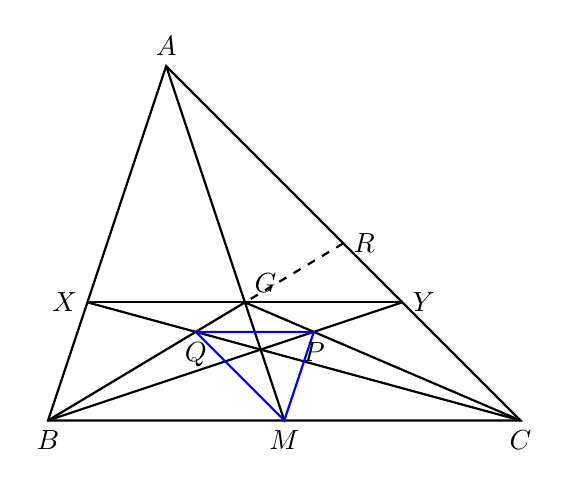
\begin{tikzpicture}
\draw[thick] (0,0) node[anchor=north] {$B$} -- (1.5,4.5) node[anchor=south] {$A$} -- (6,0) node[anchor=north] {$C$} -- cycle;
\draw[thick] (1.5,4.5) -- (3,0) node[anchor=north] {$M$};
\draw[thick] (0.5,1.5) node[anchor=east] {$X$} -- (4.5,1.5) node[anchor=west] {$Y$};
\draw (2.5,1.5) node[anchor=south west] {$G$};
\draw[thick] (0.5,1.5) -- (6,0);
\draw[thick] (2.5,1.5) -- (0,0);
\draw[thick] (4.5,1.5) -- (0,0);
\draw[thick] (2.5,1.5) -- (6,0);
\draw[thick,blue] (1.875,1.125) node[anchor=north,black] {$Q$} -- (3,0) -- (3.375,1.125) node[anchor=north,black] {$P$} -- cycle;
\draw[thick,dashed] (3.75,2.25) node[anchor=west] {$R$} -- (2.5,1.5);
\end{tikzpicture}
\end{center}

It is well known that $\frac{AG}{AM} = \frac23$; thus the ratio of the similarity between $AXY$ and $ABC$ is $\frac23$. Hence $GX = \frac12XY = \frac 13BC$.

Now look at the similarity between triangles $PBC$ and $PGX$:
\[\frac{QG}{QB} = \frac{GX}{BC} = \frac13 \implies QB = 3QG \implies QB = \frac34BG = \frac34\cdot\frac23BR = \frac12BR.\]

Finally, since $\frac{BM}{BC} = \frac{BQ}{BS}$, $MQ$ is a midline in $BCR$. Therefore $MQ = \frac12CR = \frac14AC$ and $MQ\parallel AC$. Similarly, $MP = \frac14AB$ and $MP\parallel AB$. This is sufficient to establish that $MPQ$ and $ABC$ are similar (with similarity ratio $\frac14$).

\soln
Let $S$ and $R$ be the midpoints of $AB$ and $AC$, respectively. Since $G$ is the centroid, it lies in the medians $BR$ and $CS$.
\begin{center}
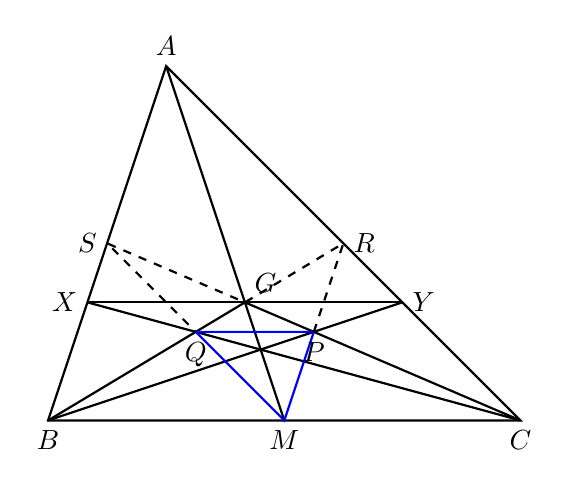
\begin{tikzpicture}
\draw[thick] (0,0) node[anchor=north] {$B$} -- (1.5,4.5) node[anchor=south] {$A$} -- (6,0) node[anchor=north] {$C$} -- cycle;
\draw[thick] (1.5,4.5) -- (3,0) node[anchor=north] {$M$};
\draw[thick] (0.5,1.5) node[anchor=east] {$X$} -- (4.5,1.5) node[anchor=west] {$Y$};
\draw (2.5,1.5) node[anchor=south west] {$G$};
\draw[thick] (0.5,1.5) -- (6,0);
\draw[thick] (2.5,1.5) -- (0,0);
\draw[thick] (4.5,1.5) -- (0,0);
\draw[thick] (2.5,1.5) -- (6,0);
\draw[thick,blue] (1.875,1.125) node[anchor=north,black] {$Q$} -- (3,0) -- (3.375,1.125) node[anchor=north,black] {$P$} -- cycle;
\draw[thick,dashed] (3.375,1.125) -- (3.75,2.25) node[anchor=west] {$R$} -- (2.5,1.5) -- (0.75,2.25) node[anchor=east] {$S$} -- (1.875,1.125);
\end{tikzpicture}
\end{center}

Due to the similarity between triangles $QBC$ and $QGX$ (which is true because $GX\parallel BC$), there is an inverse homothety with center $Q$ and ratio $-\frac{XG}{BC} = \frac{XY}{2BC}$ that takes $B$ to $G$ and $C$ to $X$. This homothety takes the midpoint $M$ of $BC$ to the midpoint $K$ of $GX$.

Now consider the homothety that takes $B$ to $X$ and $C$ to $G$. This new homothety, with ratio $\frac{XY}{2BC}$, also takes $M$ to $K$. Hence lines $BX$ (which contains side $AB$), $CG$ (which contains the median $CS$), and $MK$ have a common point, which is $S$. Thus $Q$ lies on midline $MS$.

The same reasoning proves that $P$ lies on midline $MR$. Since all homothety ratios are the same, $\frac{MQ}{MS} = \frac{MP}{MR}$, which shows that $MPQ$ is similar to $MRS$, which in turn is similar to $ABC$, and we are done.

% Problem 2
\prob Suppose there are $997$ points given in a plane. If every two points are joined by a line segment with its midpoint coloured in red, show that there are at least $1991$ red points in the plane. Can you find a special case with exactly $1991$ red points?

\sol
Embed the points in the cartesian plane such that no two points have the same $y$-coordinate. Let $P_1,P_2,\ldots,P_{997}$ be the points and $y_1 < y_2 < \ldots < y_{997}$ be their respective $y$-coordinates. Then the $y$-coordinate of the midpoint of $P_iP_{i+1}$, $i=1,2,\ldots,996$ is $\frac{y_i+y_{i+1}}2$ and the $y$-coordinate of the midpoint of $P_iP_{i+2}$, $i=1,2,\ldots,995$ is $\frac{y_i+y_{i+2}}2$. Since
\[\frac{y_1+y_2}2 < \frac{y_1+y_3}2 < \frac{y_2+y_3}2 < \frac{y_2+y_4}2 < \cdots < \frac{y_{995}+y_{997}}2 < \frac{y_{996}+y_{997}}2,\]
there are at least $996+995=1991$ distinct midpoints, and therefore at least $1991$ red points.

The equality case happens if we take $P_i = (0,2i)$, $i=1,2,\ldots,997$. The midpoints are $(0,i+j)$, $1\le i < j \le 997$, which are the points $(0,k)$ with $1+2 = 3 \le k \le 996+997 = 1993$, a total of $1993-3+1=1991$ red points.

% Problem 3
\prob Let $a_1,a_2,\ldots,a_n$, $b_1,b_2,\ldots,b_n$ be positive real numbers such that $a_1+a_2+\cdots+a_n = b_1+b_2+\cdots+b_n$. Show that
\[\frac{a_1^2}{a_1+b_1} + \frac{a_2^2}{a_2+b_2} + \cdots + \frac{a_n^2}{a_n+b_n} \ge \frac{a_1+a_2+\cdots+a_n}2.\]

\sol
By the Cauchy-Schwartz inequality,
\[\left(\frac{a_1^2}{a_1+b_1} + \frac{a_2^2}{a_2+b_2} + \cdots + \frac{a_n^2}{a_n+b_n}\right)((a_1+b_1) + (a_2+b_2) + \cdots + (a_n+b_n)) \ge (a_1+a_2+\cdots+a_n)^2.\]

Since $((a_1+b_1) + (a_2+b_2) + \cdots + (a_n+b_n)) = 2(a_1+a_2+\cdots+a_n)$,
\[\frac{a_1^2}{a_1+b_1} + \frac{a_2^2}{a_2+b_2} + \cdots + \frac{a_n^2}{a_n+b_n} \ge \frac{(a_1+a_2+\cdots+a_n)^2}{2(a_1+a_2+\cdots+a_n)} = \frac{a_1+a_2+\cdots+a_n}2.\]

% Problem 4
\prob During a break, $n$ children at school sit in a circle around their teacher to play a game.  The teacher walks clockwise close to the children and hands out candies to some of them according to the following rule. He selects one child and gives him a candy, then he skips the next child and gives a candy to the next one, then he skips $2$ and gives a candy to the next one, then he skips $3$, and soon. Determine the values of $n$ for which eventually, perhaps after many rounds, all children will have at least one candy each.

\ans All powers of $2$.

\soln
Number the children from $0$ to $n-1$. Then the teacher hands candy to children in positions $f(x) = 1 + 2 + \cdots + x\bmod n = \frac{x(x+1)}2\bmod n$. Our task is to find the range of $f\colon \mathbb{Z}_n \to \mathbb{Z}_n$, and to verify whether the range is $\mathbb{Z}_n$, that is, whether $f$ is a bijection.

If $n = 2^am$, $m>1$ odd, look at $f(x)$ modulo $m$. Since $m$ is odd, $m \mid f(x)\iff m\mid x(x+1)$. Then, for instance, $f(x) \equiv 0\pmod m$ for $x=0$ and $x=m-1$. This means that $f(x)$ is not a bijection modulo $m$, and there exists $t$ such that $f(x)\not\equiv t\pmod m$ for all $x$. By the Chinese Remainder Theorem, 
\[f(x) \equiv t \pmod n\iff
\left\{\begin{split}
f(x)\equiv t\pmod{2^a}\\
f(x)\equiv t\pmod m
\end{split}\right.\]

Therefore, $f$ is not a bijection modulo $n$.

If $n=2^a$, then
\[f(x)-f(y) = \frac12(x(x+1) - y(y+1)) = \frac12(x^2-y^2 + x-y) = \frac{(x-y)(x+y+1)}2.\]
and
\[f(x)\equiv f(y)\pmod{2^a} \iff (x-y)(x+y+1) \equiv 0\pmod{2^{a+1}}.\eqno{(*)}\]

If $x$ and $y$ have the same parity, $x+y+1$ is odd and $(*)$ is equivalent to $x\equiv y\pmod{2^{a+1}}$. If $x$ and $y$ have different parity,
\[(*)\iff x+y+1\equiv 0\pmod{2^{a+1}}.\]

However, $1\le x+y+1 \le 2(2^a-1) + 1 = 2^{a+1}-1$, so $x+y+1$ is not a multiple of $2^{a+1}$. Therefore $f$ is a bijection if $n$ is a power of $2$.

\soln
We give a full description of $a_n$, the size of the range of $f$.

Since congruences modulo $n$ are defined, via Chinese Remainder Theorem, by congruences modulo $p^\alpha$ for all prime divisors $p$ of $n$ and $\alpha$ being the number of factors $p$ in the factorization of $n$, $a_n = \prod_{p^\alpha\parallel n} a_{p^\alpha}$.

Refer to the first solution to check the case $p=2$: $a_{2^\alpha} = 2^\alpha$.

For an odd prime $p$,
\[f(x) = \frac{x(x+1)}2 = \frac{(2x+1)^2 - 1}8,\]
and since $p$ is odd, there is a bijection between the range of $f$ and the quadratic residues modulo $p^\alpha$, namely $t \mapsto 8t+1$. So $a_{p^\alpha}$ is the number of quadratic residues modulo $p^\alpha$.

Let $g$ be a primitive root of $p^\alpha$. Then there are $\frac12\phi(p^\alpha) = \frac{p-1}2\cdot p^{\alpha-1}$ quadratic residues that are coprime with $p$: $1,g^2,g^4,\ldots,g^{\phi(p^n)-2}$. If $p$ divides a quadratic residue $kp$, that is, $x^2 \equiv kp\pmod{p^\alpha}$, $\alpha \ge 2$, then $p$ divides $x$ and, therefore, also $k$. Hence $p^2$ divides this quadratic residue, and these quadratic residues are $p^2$ times each quadratic residue of $p^{\alpha-2}$. Thus
\[a_{p^\alpha} = \frac{p-1}2\cdot p^{\alpha-1} + a_{p^\alpha-2}.\]

Since $a_p = \frac{p-1}2 + 1$ and $a_{p^2} = \frac{p-1}2\cdot p + 1$, telescoping yields
\[a_{p^{2t}} = \frac{p-1}2(p^{2t-1} + p^{2t-3} + \cdots + p) + 1 = \frac{p(p^{2t}-1)}{2(p+1)} +1\]
and
\[a_{p^{2t-1}} = \frac{p-1}2(p^{2t-2} + p^{2t-4} + \cdots + 1) + 1 = \frac{p^{2t}-1}{2(p+1)} +1\]

Now the problem is immediate: if $n$ is divisible by an odd prime $p$, $a_{p^\alpha} < p^\alpha$ for all $\alpha$, and since $a_t \le t$ for all $t$, $a_n < n$.

% Problem 5
\prob Given are two tangent circles and a point $P$ on their common tangent perpendicular to the lines joining their centres. Construct with ruler and compass all the circles that are tangent to these two circles and pass through the point $P$.

\sol
Throughout this problem, we will assume that the given circles are \emph{externally} tangent, since the problem does not have a solution otherwise.

Let $\Gamma_1$ and $\Gamma_2$ be the given circles and $T$ be their tangency point. Suppose $\omega$ is a circle that is tangent to $\Gamma_1$ and $\Gamma_2$ and passes through $P$.

Now invert about point $P$, with radius $PT$. Let any line through $P$ that cuts $\Gamma_1$ do so at points $X$ and $Y$. The power of $P$ with respect to $\Gamma_1$ is $PT^2 = PX\cdot PY$, so $X$ and $Y$ are swapped by this inversion. Therefore $\Gamma_1$ is mapped to itself in this inversion. The same applies to $\Gamma_2$. Since circle $\omega$ passes through $P$, it is mapped to a line tangent to the images of $\Gamma_1$ (itself) and $\Gamma_2$ (also itself), that is, a common tangent line. This common tangent cannot be $PT$, as $PT$ is also mapped to itself. Since $\Gamma_1$ and $\Gamma_2$ have exactly other two common tangent lines, there are two solutions: the inverses of the tangent lines.
\begin{center}
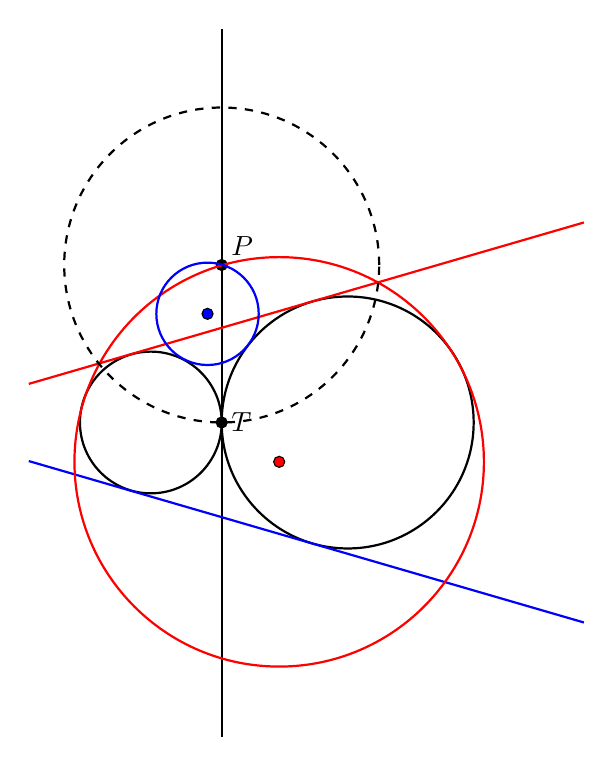
\begin{tikzpicture}
\draw[thick] (0,0) circle (0.9);
\draw[thick] (2.5,0) circle (1.6);
\draw[thick] (0.9,5) -- (0.9,-4);
\draw[thick,red] (-1.55,0.49) -- (5.5,2.54);
\draw[thick,blue] (-1.55,-0.49) -- (5.5,-2.54);
\draw[fill=black] (0.9,2) circle (2pt) node[anchor=south west] {$P$};
\draw[fill=black] (0.9,0) circle (2pt) node[anchor=west] {$T$};
\draw[thick,red] (1.63,-0.5) circle (2.6);
\draw[fill=red] (1.63,-0.5) circle (2pt);
\draw[thick,blue] (0.72,1.38) circle (0.65);
\draw[fill=blue] (0.72,1.38) circle (2pt);
\draw[thick,dashed] (0.9,2) circle (2);
\end{tikzpicture}
\end{center}

We proceed with the construction with the aid of some macro constructions that will be detailed later.
\begin{description}
\item[\bf Step 1.] Draw the common tangents to $\Gamma_1$ and $\Gamma_2$.
\item[\bf Step 2.] For each common tangent $t$, draw the projection $P_t$ of $P$ onto $t$.
\item[\bf Step 3.] Find the inverse $P_1$ of $P_t$ with respect to the circle with center $P$ and radius $PT$.
\item[\bf Step 4.] $\omega_t$ is the circle with diameter $PP_1$.
\end{description}

Let's work out the details for steps 1 and 3. Steps 2 and 4 are immediate.

\smallskip
\textbf{Step 1.} In this particular case in which $\Gamma_1$ and $\Gamma_2$ are externally tangent, there is a small shortcut:
\begin{itemize}
\item Draw the circle with diameter on the two centers $O_1$ of $\Gamma_1$ and $O_2$ of $\Gamma_2$, and find its center $O$.
\item Let this circle meet common tangent line $OP$ at points $Q,R$. The required lines are the perpendicular to $OQ$ at $Q$ and the perpendicular to $OR$ at $R$.
\end{itemize}

\begin{center}
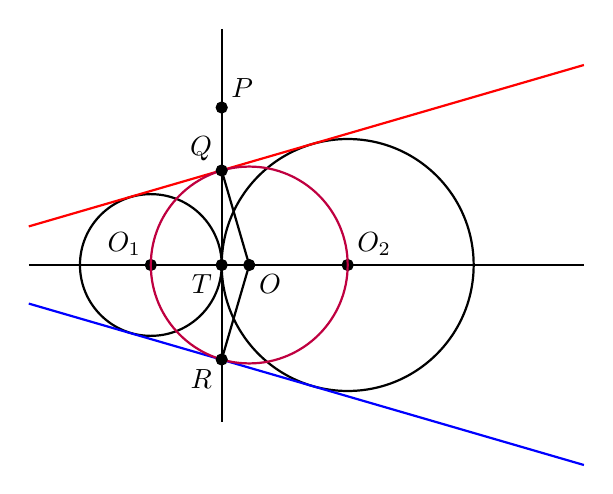
\begin{tikzpicture}
\draw[thick] (0,0) circle (0.9);
\draw[fill=black] (0,0) circle (2pt) node[anchor=south east] {$O_1$};
\draw[thick] (2.5,0) circle (1.6);
\draw[fill=black] (2.5,0) circle (2pt) node[anchor=south west] {$O_2$};
\draw[thick] (0.9,3) -- (0.9,-2);
\draw[thick] (-1.55,0) -- (5.5,0);
\draw[thick,red] (-1.55,0.49) -- (5.5,2.54);
\draw[thick,blue] (-1.55,-0.49) -- (5.5,-2.54);
\draw[fill=black] (0.9,2) circle (2pt) node[anchor=south west] {$P$};
\draw[fill=black] (0.9,0) circle (2pt) node[anchor=north east] {$T$};
\draw[thick,purple] (1.25,0) circle (1.25);
\draw[fill=black] (1.25,0) circle (2pt) node[anchor=north west] {$O$};
\draw[fill=black] (0.9,1.2) circle (2pt) node[anchor=south east] {$Q$};
\draw[fill=black] (0.9,-1.2) circle (2pt) node[anchor=north east] {$R$};
\draw[thick] (0.9,1.2) -- (1.25,0) -- (0.9,-1.2);
\end{tikzpicture}
\end{center}

Let's show why this construction works. Let $R_i$ be the radius of circle $\Gamma_i$ and suppose without loss of generality that $R_1 \le R_2$. Note that $OQ = \frac12 O_1O_2 = \frac{R_1+R_2}2$, $OT = OO_1 - R_1 = \frac{R_2-R_1}2$, so
\[\sin\angle TQO = \frac{OT}{OQ} = \frac{R_2-R_1}{R_1+R_2},\]
which is also the sine of the angle between $O_1O_2$ and the common tangent lines.

Let $t$ be the perpendicular to $OQ$ through $Q$. Then $\angle(t,O_1O_2) = \angle(OQ,QT) = \angle TQO$, and $t$ is parallel to a common tangent line. Since
\[d(O,t) = OQ = \frac{R_1+R_2}2 = \frac{d(O_1,t)+d(O_2,t)}2,\]
and $O$ is the midpoint of $O_1O_2$, $O$ is also at the same distance from $t$ and the common tangent line, so these two lines coincide.

\smallskip
\textbf{Step 3.} Finding the inverse of a point $X$ given the inversion circle $\Omega$ with center $O$ is a well known procedure, but we describe it here for the sake of completeness.
\begin{itemize}
\item If $X$ lies in $\Omega$, then its inverse is $X$.
\item If $X$ lies in the interior of $\Omega$, draw ray $OX$, then the perpendicular line $\ell$ to $OX$ at $X$. Let $\ell$ meet $\Omega$ at a point $Y$. The inverse of $X$ is the intersection $X'$ of $OX$ and the line perpendicular to $OY$ at $Y$. This is because $OYX'$ is a right triangle with altitude $YX$, and therefore $OX\cdot OX' = OY^2$.
\item If $X$ is in the exterior of $\Omega$, draw ray $OX$ and one of the tangent lines $\ell$ from $X$ to $\Omega$ (just connect $X$ to one of the intersections of $\Omega$ and the circle with diameter $OX$). Let $\ell$ touch $\Omega$ at a point $Y$. The inverse of $X$ is the projection $X'$ of $Y$ onto $OX$. This is because $OYX'$ is a right triangle with altitude $YX'$, and therefore $OX\cdot OX' = OY^2$.
\end{itemize}

\begin{center}
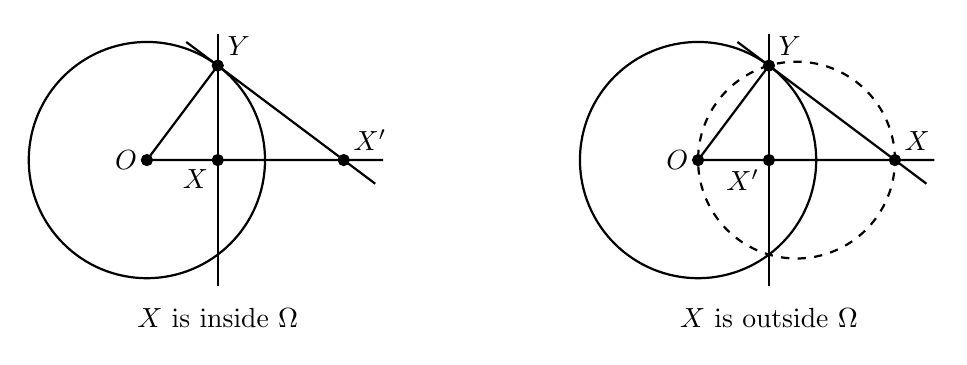
\begin{tikzpicture}
% Diagram 1
\draw[thick] (0,0) circle (1.5);
\draw[fill=black] (0,0) circle (2pt) node[anchor=east] {$O$};
\draw[fill=black] (2.5,0) circle (2pt) node[anchor=south west] {$X'$};
\draw[fill=black] (0.9,0) circle (2pt) node[anchor=north east] {$X$};
\draw[fill=black] (0.9,1.2) circle (2pt) node[anchor=south west] {$Y$};
\draw[thick] (0.9,1.6) -- (0.9,-1.6);
\draw[thick] (3,0) -- (0,0) -- (0.9,1.2);
\draw[thick] (0.5,1.5) -- (2.9,-0.3);
\draw (0.9,-2) node {$X$ is inside $\Omega$};
% Diagram 2
\draw[thick] (7,0) circle (1.5);
\draw[dashed, thick] (8.25,0) circle (1.25);
\draw[fill=black] (7,0) circle (2pt) node[anchor=east] {$O$};
\draw[fill=black] (9.5,0) circle (2pt) node[anchor=south west] {$X$};
\draw[fill=black] (7.9,0) circle (2pt) node[anchor=north east] {$X'$};
\draw[fill=black] (7.9,1.2) circle (2pt) node[anchor=south west] {$Y$};
\draw[thick] (7.9,1.6) -- (7.9,-1.6);
\draw[thick] (10,0) -- (7,0) -- (7.9,1.2);
\draw[thick] (7.5,1.5) -- (9.9,-0.3);
\draw (7.9,-2) node {$X$ is outside $\Omega$};
\end{tikzpicture}
\end{center}

\end{document}